\documentclass[12pt,a4paper,twoside]{article}
\usepackage{fancyhdr,graphicx,latexsym}

\setlength{\parindent}{0cm}
\setlength{\parskip}{2ex plus1ex minus 0.5ex}

\addtolength{\evensidemargin}{-2.5cm}
\addtolength{\oddsidemargin}{-0.5cm}
\addtolength{\textwidth}{3cm}

\addtolength{\headheight}{0.2cm}
\addtolength{\topmargin}{-1cm}
\addtolength{\textheight}{2.5cm}

\renewcommand{\_}{\texttt{\symbol{95}}}
\addtolength{\fboxsep}{0.1cm}
\newcommand{\param}[1]{\textit{\textrm{\textmd{#1}}}}
\newcommand{\codebar}{\rule{\textwidth}{0.3mm}}
% \newcommand{\spc}{\hspace{0.5mm}$\sqcup$\hspace{0.6mm}}
\newcommand{\spc}{\hspace{0.5mm}$\Box$\hspace{0.5mm}}
\newcommand{\todo}[1]{\textbf{TODO: #1}}

\newlength{\codelen}
\newcommand{\code}[1]
{\begin{center}\fbox{\parbox{16cm}{\texttt{#1}}}\end{center}}

\fancyhead{}
\fancyhead[RO,LE]{\thepage}
\fancyhead[LO,RE]{SBUS Dynamics}
\fancyfoot{}
\pagestyle{empty}

\newenvironment{bulletlist}
{
	\begin{itemize}
	\setlength{\itemsep}{0ex}
	\setlength{\parsep}{0ex}
}
{
	\end{itemize}
}

\newenvironment{alphalist}
{
	\begin{enumerate}
	\setlength{\itemsep}{0ex}
	\setlength{\parsep}{0ex}
	\renewcommand{\labelenumi}{(\alph{enumi})}
}
{
	\end{enumerate}
}

\newenvironment{numericlist}
{
	\begin{enumerate}
	\setlength{\itemsep}{0ex}
	\setlength{\parsep}{0ex}
}
{
	\end{enumerate}
}

\begin{document}

% \sfseries
\centerline{\textbf{\LARGE SBUS Dynamics}}
\vspace{3mm}
\centerline{\textbf{\LARGE Preliminary Draft}}
\begin{center} \large
David Ingram\\
TIME-EACM Project\\
University of Cambridge Computer Lab\\
3rd September 2007\\
\end{center}

{ \parskip 1mm plus 1pt \tableofcontents }
\pagestyle{fancy}

\vspace{10mm}
\fbox{\parbox{16cm}{\textit{\textbf{Warning:} this document contains
preliminary ideas only.}}}

\section{Flow control}

\subsection{Detecting overload}

Flow control applies to source/sink endpoints only.
Contra-flow acknowledgement messages are used to signify completed
end-to-end processing of previous messages. The source must pause
sending data when it is awaiting the return of \textit{more than one}
acknowledgement of its earlier messages (it is always OK to continue
with one outstanding acknowledgement).%
\footnote{We rejected a mechanism based on ``slow down'' messages
because these may not get through during overload. We also rejected
characterising conditions such as out-of-CPU on the client,
out-of-bandwidth on the link, out-of-TCP buffer space, and out-of-CPU
on the server.
It's better to use an end-to-end indicator of successful flow.}

Flow control policy parameter:
\begin{bulletlist}
\item \texttt{b} -- Acknowledge every \texttt{b} bytes of data.
   The acknowledgement is sent after a message takes the cumulative
   amount of data seen since the last acknowledgement above the limit.
   The counter is then reset to zero.
\end{bulletlist}

This parameter is set by the subscriber for pull-stream connections,
and by the receiver for push-streams. The first acknowledgement is due
after a single byte of data. The parameter can then be changed
by specifying it in the acknowledgement packet itself.

\subsection{Recovery from overload}
\label{overload-policy}

In the presence of overload, some real time streams need to drop
messages in order to stay up to date and hence degrade gracefully,
whereas for others it is important that they buffer them all
(or as many as possible) and replay every message later at a slower rate.

Overload policy parameters:
\begin{bulletlist}
\item \texttt{B} -- Maximum number of bytes to buffer.
\item \texttt{t} -- Maximum age of messages to keep (in ms).
\end{bulletlist}

Events are dropped once either of these conditions are reached.
After this, \textit{older} events are discarded, not newer ones.
The parameters apply to the publisher for push-streams, and to
the notifier for pull-streams.

Option to inform the component and/or the client about\\
-- temporary overload?\\
-- events being dropped?\\
-- buffer overflow whilst disconnected?\\

\section{Timeouts}

\begin{bulletlist}
\item Connection establishment timeout
\item Connection closure timeout
\item No response / acknowledgement timeout
\item RPC processing timeout
\item Incomplete message timeout
\end{bulletlist}

\section{Dynamic reconfiguration objectives}

Dynamic reconfiguration allows the communication links between components
to be rewired whilst the components continue to run. There are several
desirable properties to be observed:

\begin{bulletlist}
\item Don't miss any messages (at least once semantics)
\item Don't replay any messages twice (at most once semantics)
\item Don't delay any messages for too long during reconfiguration
\item Don't interrupt suppliers or consumers of the reconfigured
		components
\end{bulletlist}

For each of these properties, there are some applications which can tolerate
them and others which cannot. There are also applications which can tolerate
skipping messages but for a short period of time only.

\section{Dynamic reconfiguration primitives}

\subsubsection*{Connection flags}

\begin{bulletlist}
\item \textbf{Await transfer} open connection flag.\\
	This indicates that the client wishes to connect but not to
	receive any messages until another client has departed and
	transferred its assets.
\end{bulletlist}

\subsubsection*{Endpoints}

\begin{bulletlist}
\item \verb^migrate(new_address)^\\
	Triggers the migration process
\item Lower-level endpoints to request freeze, unfreeze, divert or transfer?
\item Endpoints to get and set sequence numbers?
\end{bulletlist}

\subsubsection*{OOB messages}

\begin{bulletlist}
\item \verb^freeze^ (client to server)\\
	Instructs the server to start buffering messages which would have
	been delivered to this client instead of sending them. Messages
	are not discarded unless the server runs out of buffer space.
	This only freezes the connection to this client, not the whole
	server component.
\item \verb^divert(address)^ (server to client)\\
	Instructs clients to move to another server. The server
	sending this instruction will close the connection immediately afterwards.
\item \verb^transfer(address)^ (client to server)\\
	This instruction is typically applied to a frozen endpoint.
	Connections from the server are switched from the current client
	to another named client. This is atomic so no data is lost in between.
	If the connection is currently frozen, the buffered messages are
	now played out to the new client.
	The client which loses its connection ends up with an endpoint in
	the unmapped state.
\item \verb^unfreeze^ (client to server)\\
	Resume sending to the same client as before (plays out buffered
	messages first).
\end{bulletlist}

\subsubsection*{Freezing data sources}

\subsubsection*{Source \textit{transfers}}

\subsubsection*{Holding state for incoming (?) requests}

In the holding state all output (?) streams are paused. Uses include
upgrading components to a newer version.

\section{Migration}

In its simplest form, components could move to a different address by
terminating, restarting elsewhere and re-registering with the resource
discovery service (doing so breaks any current connections to the component and
loses messages until the clients reconnect, of course).

SBUS also supports seamless migration. A packet with the message type
\texttt{divert} indicates the component is about to migrate. The message
contents supply the new location.

\begin{figure}[h]
\centering
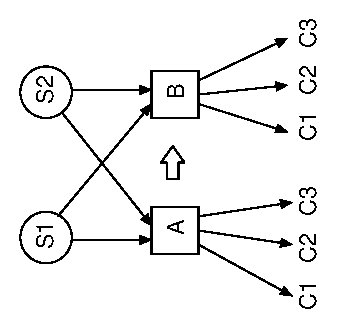
\includegraphics[scale=1.0,angle=-90]{diagrams/migration.eps}
\caption{Component migration}
\label{migration}
\end{figure}

\textbf{Migration procedure:}

\begin{tabular}{ll}
1 & Start B, with endpoint awaiting transfer\\
2 & Call \verb^migrate(B's address)^ SAP on A\\
3 & Freeze A's inputs\\
4 & Stop advertising A on RDC\\
5 & A stops accepting new connections\\
6 & Flush A's processing\\
7 & Divert A's clients to B\\
8 & Transfer A's inputs to B\\
9 & Kill A\\
\end{tabular}

\section{Upgrading components}

Component upgrading is defined as replacing a component with an internally
improved version which has identical API's. The new version might improve
performance or fix bugs, for example. The mechanism used is identical to that
for component migration (see the previous section).

\section{Automatic reconnection}

Automatic reconnection is initiated if a mapped component fails
(disconnects unexpectedly). Note that server components take no action if
their \textit{clients} exit ungracefully.
Reconnection is only attempted by a component's wrapper when a mapped
server, source or sink departs unexpectedly.

Policies:

\begin{bulletlist}
\item Reconnect automatically without bothering application
	\begin{bulletlist}
	\item To same address
	\item To a different address (check RDC)
	\item To a different component (remap contact)
	\end{bulletlist}
\item Warn application and try to reconnect
\item Don't try to reconnect; just return a disconnected error
\end{bulletlist}

\subsection{Failover}

\todo{How does this work?}

Failover and migration both require stream item sequence numbers
(as distinct from connection sequence numbers)...

\subsection{Lost events}

Stream sources may choose to buffer events whilst disconnected and
to replay them once reconnected, or to simply discard events
whilst disconnected. In the former case the overload policy (see
\S \ref{overload-policy}) is used to determine how much can be
buffered.

\begin{bulletlist}
\item Buffer events until reconnected, then replay
\item Drop events whilst disconnected, don't replay
\end{bulletlist}

N.B. Application semantics may mean that lost events can be summarised,
e.g. by just transmitting the final state. This is best handled by
declining replay, and calling a \texttt{get\_app\_status}
RPC after restarting
to initialise before resuming listening to the stream.

\subsection{Common output buffer}

All streams have a time-window output buffer. This can be used for replay
when a client comes back up, and when a client is stalled due to flow
control.

\subsection{Intermediate machine failure}

Suppose B is a client of a stream from A, and C is a client of a
stream from B. We wish to ensure that C sees all the messages
derived from A's output.

When B crashes, A must buffer data so it can be replayed when
B reconnects.

We could achieve this by always buffering say 3 minutes of output
for all source endpoints. Better: \verb^n^ secs or \verb^m^ KB, whichever
is lower.
We can have a common output buffer, and all clients awaiting data
from it can have a queue of message ID's. (But not if a pull-stream
allows different subscription parameters).

Difficult case: what if a physical machine hosting several different
components which supply each other in a subgraph crashes?

Failure recovery can be assisted by calling the \verb^get_connections^
endpoint on remaining components and examining \verb^lastseq^
to discover at what point in the stream connections were broken.

\section{Replication}

SBUS supports multiple instances of a given component. They all have
the same name, but different locations (IP address / port). Each one is
listed with a separate \verb^status^ block in the component metadata by
the RDC. Each instance must supply the correct authorisation when
registering with the RDC (normally they will all be exactly the same
program, running on different machines, but the only requirements are
that they implement the component's API and supply implementor's
authorisation matching that in the component's metadata).

\subsection{Starting a new replica}

\subsection{Load balancing}

The \verb^status^ block for each component replica contains the load
information last reported by that component. Clients may choose any
replica, for example based on ping time, or IP address. If not
specified the default policy is to select whichever is estimated to be
the least loaded, a function which is computed from recent message
counts, machine CPU usage and occurrences of flow control.

Policies:

\begin{bulletlist}
\item random
\item least ping time
\item least average request latency
\item least loaded (CPU)
\item least dropped events
\item fewest clients
\item a function of all the above (pass a pointer to a scoring function which
	takes the load metadata structure as an argument)
\end{bulletlist}

\section{Evolution of data formats and API's}

It is typical for message formats to change throughout the lifetime of
a project. New fields may be added, old ones removed, they may be
renamed, the range of values used in a field may be altered, and their
meaning (semantics) may change. Any of these changes will cause new
LITMUS codes to be used. This shows that the new type is generally
incompatible with the old one (except for the case of just adding new
fields, which is dealt with by the partial matching extension).

One method for dealing with incompatible API changes is to
create adapters (event transformers) as other components.
It is also possible to create components which register multiple
endpoints with the \textit{same} name but \textit{different} API hashes
(like Facets In ICE).

Q. How to transition from old to new data formats without stopping
the stream?

\subsubsection*{Stategy 1}

Upgrade all clients to cope with both V1 and V2\\
Upgrade V1 server to V2 server\\
Upgrade all clients to understand V2 only\\

This is tricky because clients have to be coded to try mapping a
V2 server, then failing that V1. Existing connections can't be
smoothly converted. It's also unrealistic to fix all clients before
the server can be upgraded in some scenarios.

\subsubsection*{Stategy 2}

Upgrade server to offer both V1 and V2 API's\\
Clients gradually upgraded from V1 clients to V2 clients\\
Upgrade server to V2 only, to drop legacy code\\

\subsubsection*{Strategy 3}

Start a separate V2 server\\
Clients gradually upgrade from V1 clients to V2 clients\\
Stop the V1 server\\

This requires component migration \textit{and} API hash change
at the second step.

\section{Dynamic reconfiguration scenarios}

\textbf{Non-terminating}
\begin{bulletlist}
\item New replica starts -- synchronisation needed
\end{bulletlist}

\textbf{Involuntary termination}
\begin{bulletlist}
\item Failover to another replica
\item Restart failed component
\item Restart failed subgraph
\end{bulletlist}

\textbf{Voluntary termination}
\begin{bulletlist}
\item Upgrade component
\item Migrate component
\item Add filter to chain
\item Reduce chain
\item Replace subgraph
\end{bulletlist}

\todo{Consider the effect of longer downtime when a machine fails}

\subsection{Reduce chain}

\begin{figure}[h]
\centering
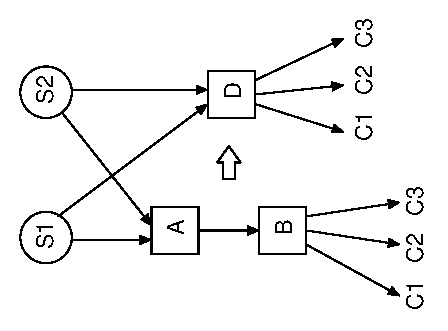
\includegraphics[scale=1.0,angle=-90]{diagrams/reduce.eps}
%\caption{Component migration}
%\label{migration}
\end{figure}

\begin{tabular}{ll}
1 & Freeze A\\
2 & Start D awaiting transfer\\
3 & Stop advertising A and B on the RDC\\
4 & A and B stop accepting new connections\\
5 & Flush A and B\\
6 & Divert clients from B to D\\
7 & Transfer A's inputs to D\\
8 & Kill A and B\\
\end{tabular}

\subsection{Insert filter (I)}

\begin{figure}[h]
\centering
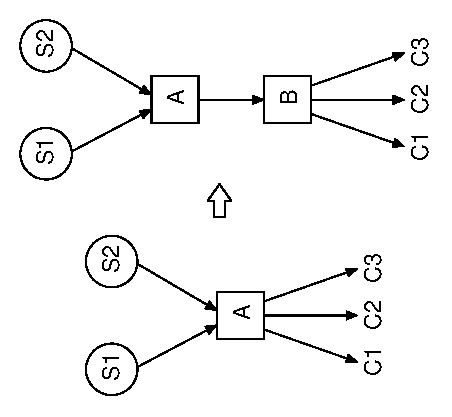
\includegraphics[scale=1.0,angle=-90]{diagrams/insert1.eps}
%\caption{Component migration}
%\label{migration}
\end{figure}

\begin{tabular}{ll}
1 & Freeze A's inputs\\
2 & Flush A\\
3 & Start B\\
4 & Divert clients from A to B\\
5 & Unfreeze A's inputs\\
\end{tabular}

\subsection{Insert filter (II)}

\begin{figure}[h]
\centering
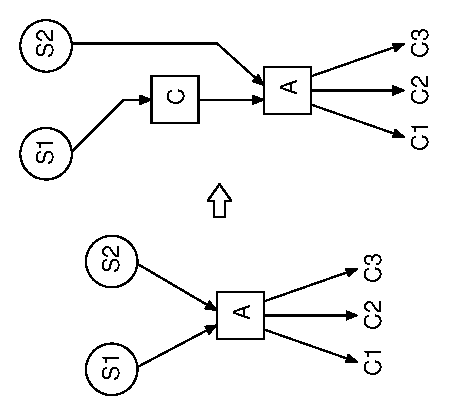
\includegraphics[scale=1.0,angle=-90]{diagrams/insert2.eps}
%\caption{Component migration}
%\label{migration}
\end{figure}

\begin{tabular}{ll}
1 & Freeze A's S1 input\\
2 & Start C awaiting transfer on input from S1\\
3 & Transfer A's S1 input to C\\
4 & Map A's now unmapped input to C\\
\end{tabular}

\subsection{Replace sub-graph}

\begin{tabular}{ll}
1 & Freeze inputs to sub-graph\\
2 & Start new sub-graph awaiting transfer on external inputs\\
3 & Stop advertising components from original sub-graph on RDC\\
4 & Stop accepting new connections to original sub-graph\\
5 & Flush processing within sub-graph\\
6 & Divert clients to new sub-graph\\
7 & Transfer external inputs between sub-graphs\\
8 & Kill original sub-graph\\
\end{tabular}

\section{Latency tracking}

For performance monitoring as well as load balancing, it is useful to
know typical round trip times.

See Figure \ref{latency}.

\begin{figure}[h]
\centering
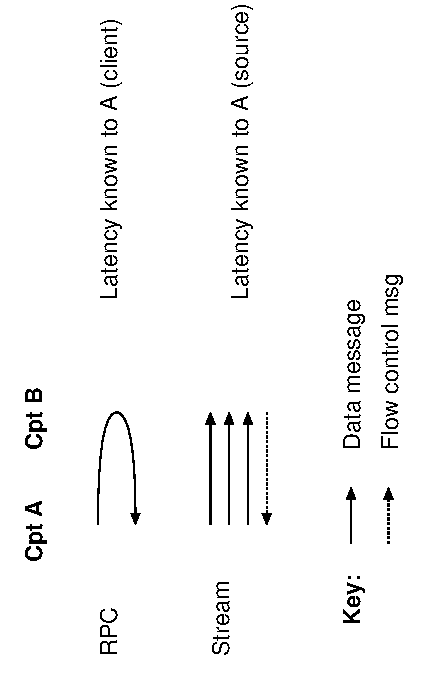
\includegraphics[scale=1.0,angle=-90]{diagrams/latency.eps}
\caption{Latency observation}
\label{latency}
\end{figure}

\section{Future work}

\subsection*{Tracer packets}

What to call them (magic strawberries / driftwood etc...)\\
Barriers, boundaries\\
Includes a recognition string\\
Scope: list of nodes (critical region)?

\end{document}
